%!TEX root = ../thesis.tex

%%%%% Chapter: Introduction %%%%%
\chapter{Introduction}

\ifpdf
    \graphicspath{{Chapter1/Figs/Raster/}{Chapter1/Figs/PDF/}{Chapter1/Figs/}}
\else
    \graphicspath{{Chapter1/Figs/Vector/}{Chapter1/Figs/}}
\fi


%%% Background %%%
\section{Background}
\label{sec:intro-background}

% filled-in handouts
In the context of CUED teaching, a common way of delivering lectures is to prepare handouts with a number of intentional gaps and fill the missing contents in these gaps during the lectures. This method is especially popular for teaching Part IA and IB courses. Usually, the scanned PDF version of the filled-in handout will be uploaded to the Moodle (also called the Virtual Learning Environment) after every lecture is finished. \Cref{fig:intro-example-handouts} shows some example scans of filled-in handout pages\footnote{Image source: CUED Part IA Mathematics (2010)}.

% latex slides
Another common way of teaching CUED courses would be using fully digital presentation slides, usually typeset by \LaTeX ~and arranged in the landscape orientation. This approach is more common in teaching Part IIA and IIB courses and is especially popular in Division F. Examples of this kind of lecture slides\footnote{Image source: CUED Part IIB 4F8: Image Processing and Image Coding} are shown in \Cref{fig:intro-example-slides}.

% panopto
In the recent years, full lecture video recordings of major CUED Part IA and IB courses have been accessible to students online via the Panopto service. The service provides the lecture video playback service with aligned handout/slide projections. With this service, Part IA and IB students are able to revisit specific parts of the lectures, which relieves them of the pressure of taking notes and understanding hard topics during lectures.

\begin{figure}[!htb]
    \centering
    \begin{subfigure}{.47\textwidth}
        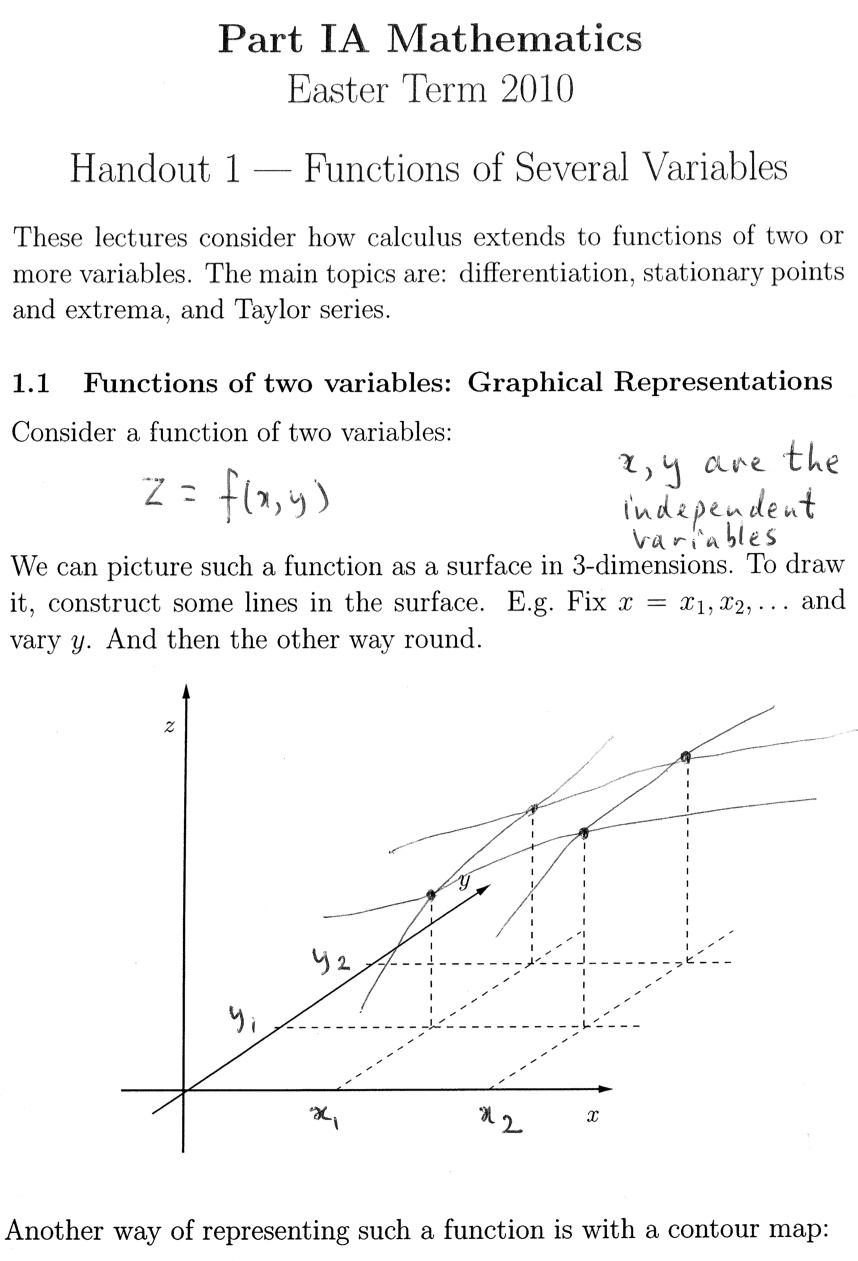
\includegraphics[width=\textwidth]{handout1.jpg}
    \end{subfigure}%
    \begin{subfigure}{.52\textwidth}
        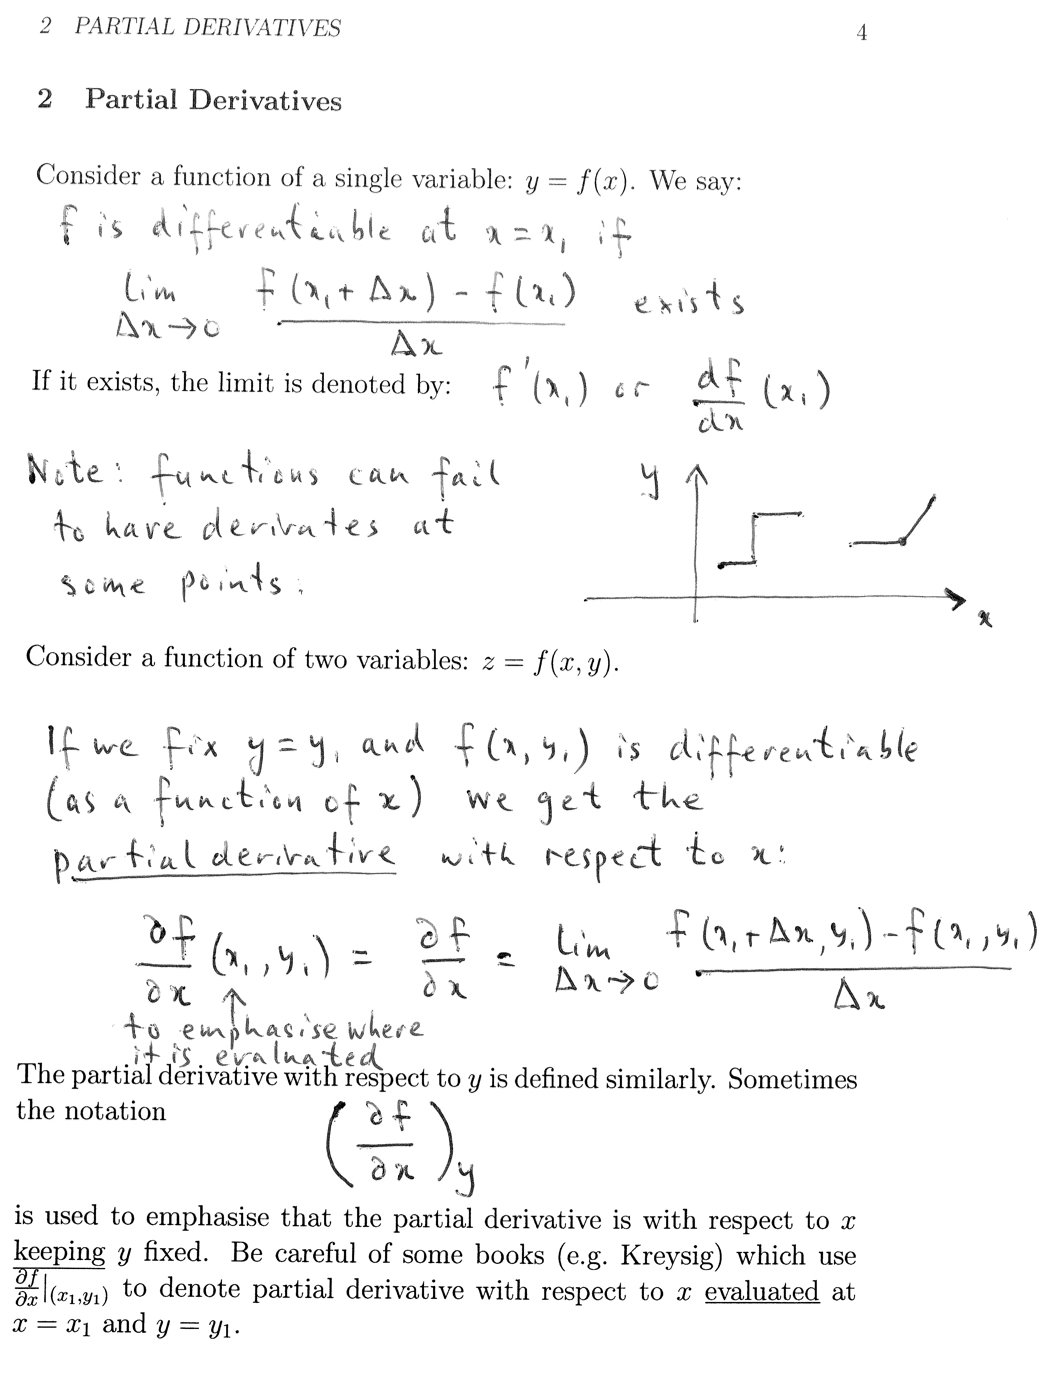
\includegraphics[width=\textwidth]{handout2.jpg}
    \end{subfigure}
    \caption{Examples of scanned handout pages with filled-in notes}
    \label{fig:intro-example-handouts}
\end{figure}

\begin{figure}[!htb]
    \centering
    \begin{subfigure}{.49\textwidth}
        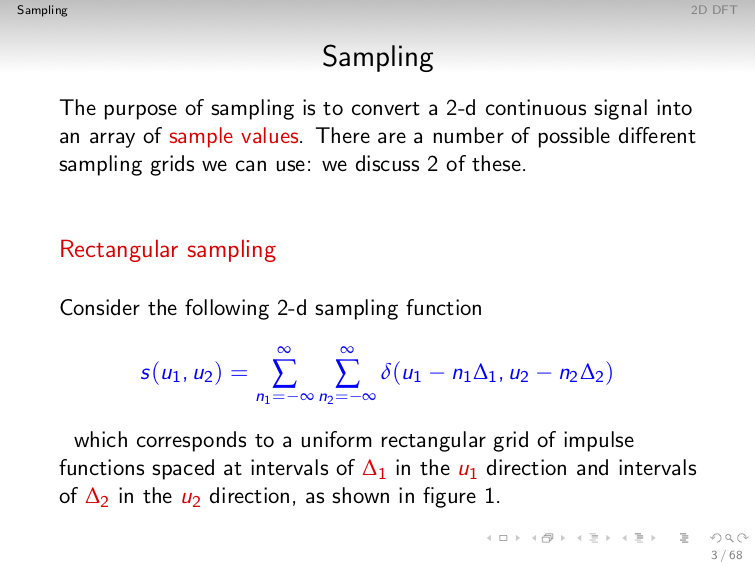
\includegraphics[width=\textwidth]{slide1.jpg}
    \end{subfigure}%
    \begin{subfigure}{.49\textwidth}
        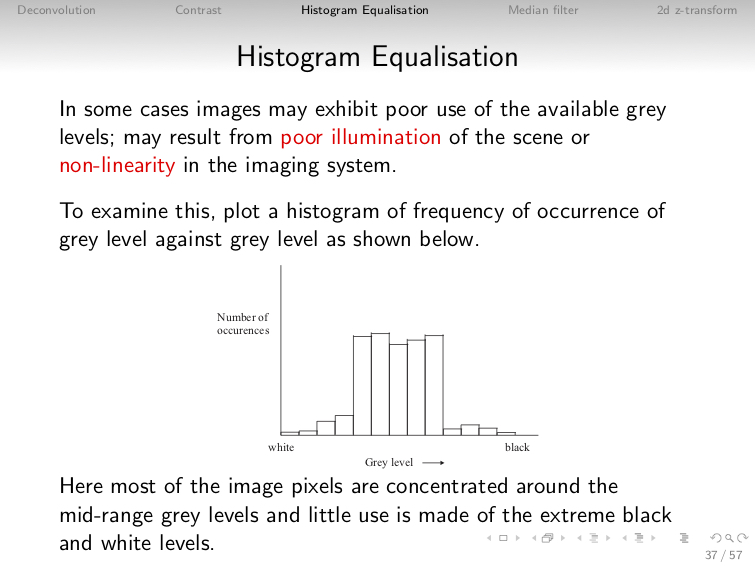
\includegraphics[width=\textwidth]{slide2.jpg}
    \end{subfigure}
    \caption{Examples of lecture slides typeset by \LaTeX}
    \label{fig:intro-example-slides}
\end{figure}


%%% Motivation %%%
\section{Motivation}

% situation
As mentioned in \Cref{sec:intro-background}, the Panopto service enables students to revisit parts of the lecture recordings, which has significantly enhanced their educational experience. A common situation for students is that they may have difficulties understanding specific parts in the handouts, such as the core concepts or some complicated equations, and they would like to refer back to lecturers' explanations to these parts. However, in order to find the correct parts of the lecture recordings that they are actually interested in, students still need to search back and forth in these recordings before they eventually arrive at the desired parts.

% ideal system
Therefore, it would be ideal to have a system which automatically analyses the lecture data (handouts + recordings) and brings us directly to the correct parts of the recordings upon selecting specific parts in the handouts. Such a system will aid the students to locate the desired parts of the recordings with minimum effort, and will even further improve their overall educational experience. The idea behind such a system is also termed as `talking handouts', which is the title of this project.

% reality
Unfortunately, few work has been done in designing and implementing such a system so there are not many useful references for this project. However, there are lots of relevant tools available such as OCR engines and speech recognisers, and it would still be interesting and worthwhile to try building a minimum working system based on these tools to test the feasibility of this idea, starting from the simplest assumptions.


%%% Project Aim
\section{Project Aims}
\label{sec:intro-aims}

% general aim
This project aims to investigate the feasibility of the idea `talking handouts' by designing, implementing and evaluating a minimum working software system which automatically computes the alignment (or mappings) between the chunks of handouts and the segments of the corresponding lecture recordings. Here we use the word `chunk' to denote a block of meaningful information in the handouts, and use the word `segment' to denote an interval with a starting time and an ending time in the lecture recordings. The wording `chunk' and `segment' will be used throughout the report.

% first subtask
The first major subtask of the project is to investigate methods of dividing the handouts into smaller chunks of information (at different scales) and extracting meaningful text from these chunks. A direct solution to this subtask is to use an OCR engine, which is adopted in the system design and further discussed in \Cref{chap:tess-ocr}.

% second subtask
The second major subtask of the project is to investigate speech-recognition based algorithms of aligning chunks of handouts with segments of lecture recordings. `Speech-recognition based' means that the lecture recordings are first fed into a speech recogniser and we use the output of the recogniser as one of the inputs of the alignment algorithm (the other input is the chunks of extracted handout text). The final system uses a \texttt{diff}-based alignment algorithm which is discussed in detail in \Cref{chap:align}.

% some assumptions
It would be worth mentioning that the project will only focus on handouts with filled-in handwritten notes (discussed in the first paragraph of \Cref{sec:intro-background}), since handouts of this type are fundamental to the CUED teaching (especially for Part IA and IB) and they also contain handwritten information which is interesting to investigate. 

In addition, the expression `speech-recognition based' in the second subtask has two further implications. The first implication is that the system is supposed to be using a mature speech recogniser and we are not going to care about how to tune the speech recogniser. The second implication is that we will only be using the audio information of the lecture recordings and the video information will be abandoned for simplicity. To avoid confusion, the wording `lecture audio file' is used instead of `lecture recording' in the rest of the report.

\section{Approach}

As a first step, basic assumptions are made on the system inputs and output. Based on these assumptions, the system architecture could then be designed. The 2 core subsystems, namely the OCR engine and the alignment algorithm, are investigated further to optimise the overall system performance, quantified by suitable metrics defined in the dedicated evaluation framework. Eventually, a GUI system is implemented to visualise the system alignment output and the results from the evaluation framework.

%%% Report Structure %%%
\section{Report Structure}

\begin{description}[leftmargin=5.5em,labelwidth=5em]
\item[Chapter 2] explains the basic assumptions on the system inputs and output
\item[Chapter 3] explains the design of the system architecture based on the basic assumptions in \Cref{chap:basic-assumptions} and briefly introduces the involved subsystems 
\item[Chapter 4] explains the Tesseract OCR engine with more detail, including the PLA and the training process
\item[Chapter 5] explains the mathematical formulation of the sequence alignment problem and how it is adapted to the actual alignment algorithm used in the system
\item[Chapter 6] explains the basic elements which support the operation of the system
\item[Chapter 7] explains how the system is evaluated
\item[Chapter 8] briefly introduces the setup of the actual software implementation
\item[Chapter 9] evaluates the system using the methodologies explained in \Cref{chap:eval-framework}
\item[Chapter 10] concludes the main findings and suggests possible future work
\end{description}


%% example nomenclatures
% \nomenclature[z-DKT]{DKT}{Draft Kiss Tumble}
% \nomenclature[z-PPC]{PPC}{Particles per cell}
\nomenclature[z-CUED]{CUED}{Cambridge University Engineering Department}
\nomenclature[z-VLE]{VLE}{Virtual Learning Environment}
\nomenclature[z-OCR]{OCR}{Optical Character Recognition}